% \iffalse meta-comment
%
% Copyright (C) 2021 by Geraldo Xexéo
%
% This file may be distributed and/or modified under the
% conditions of the LaTeX Project Public License, either
% version 1.3 of this license or (at your option) any later
% version. The latest version of this license is in:
%
% http://www.latex-project.org/lppl.txt
%
% and version 1.3 or later is part of all distributions of
% LaTeX version 2005/12/01 or later.
%
% \fi
%
%
%\iffalse
%<package>\NeedsTeXFormat{LaTeX2e}
%<package>\def\cw@version{v1.1.2}
%<package>\ProvidesPackage{coop-writing}[2021/05/18 \cw@version dtx version of coop-writing]
%<*driver>
\documentclass{ltxdoc}
\usepackage[T1]{fontenc}
\usepackage[utf8]{inputenc}
\usepackage{csquotes}
\usepackage[brazilian,english]{babel}
\usepackage{datetime}
\usepackage{indentfirst}
\usepackage{enumitem}
\usepackage{graphicx}
\setlist{noitemsep}
\setlength{\parskip}{0.5em}
\usepackage{marvosym}
\usepackage[backend=biber,style=alphabetic,natbib]{biblatex}
\addbibresource{coop-writing.bib}
\usepackage[editing]{coop-writing}
%%\usepackage{textcomp,url,a4wide,array}
%%\usepackage[eso-foot,today,draft]{svninfo}
%%\usepackage{xcolor}
\usepackage{marvosym}
\usepackage{hyperref}
\cwnamedef{xexeo}{red}{Xexéo}
%
\EnableCrossrefs
\CodelineIndex
\RecordChanges
%
\DoNotIndex{\def,\long,\edef,\xdef,\gdef,\let,\global}
\DoNotIndex{\begin,\AtEndDocument,\newcommand,\newcounter,\stepcounter}
\DoNotIndex{\immediate,\openout,\closeout,\message,\typeout}
\DoNotIndex{\section,\scshape,\arabic}
%
%
%
\title{coop-writing \coopwritingversion}
\author{Geraldo Xexéo}
\date{\today\ - \ \currenttime}
\GetFileInfo{coop-writing.sty}
%
\makeindex
\MakeShortVerb{\|}
\begin{document}
    \DocInput{coop-writing.dtx}
    \printbibliography
    \newpage
    \PrintChanges
    \newpage
    \PrintIndex
    \listofcomments
    \newpage
    \listofcitationneeds
    \newpage
    \listofsubject
\end{document}
%</driver>
% \fi
%
% \CheckSum{652}
%
% \CharacterTable
%  {Upper-case    \A\B\C\D\E\F\G\H\I\J\K\L\M\N\O\P\Q\R\S\T\U\V\W\X\Y\Z
%   Lower-case    \a\b\c\d\e\f\g\h\i\j\k\l\m\n\o\p\q\r\s\t\u\v\w\x\y\z
%   Digits        \0\1\2\3\4\5\6\7\8\9
%   Exclamation   \!     Double quote  \"     Hash (number) \#
%   Dollar        \$     Percent       \%     Ampersand     \&
%   Acute accent  \'     Left paren    \(     Right paren   \)
%   Asterisk      \*     Plus          \+     Comma         \,
%   Minus         \-     Point         \.     Solidus       \/
%   Colon         \:     Semicolon     \;     Less than     \<
%   Equals        \=     Greater than  \>     Question mark \?
%   Commercial at \@     Left bracket  \[     Backslash     \\
%   Right bracket \]     Circumflex    \^     Underscore    \_
%   Grave accent  \`     Left brace    \{     Vertical bar  \|
%   Right brace   \}     Tilde         \~}
%
% \changes{v1.0}{2021/05/29}{First version}
% \changes{v1.1}{2021/05/30}{You can put an aditional symbol before the comment superscript number} 
% \changes{v1.1.1}{2021/05/30}{Fix some bugs, anonymization back on manual} 
% \changes{v1.1.2}{2021/05/30}{PDF bookmarks can't handle full UTF} 
%\maketitle
%
% \tableofcontents
%
%\section{Introduction}
%
% This package supports editorial comments and gives some extra support for writing papers, or any document that involves more than one author or editor.
%
% Usually, a final version of a  document would be printed with the |publish| option turned one, and no editorial comment would appear.  
% In this document \xexeo[the reader will see some uses]{This is an exemple of using this package to make a comment with highlighted text} of the package, since it is distributted with the |editing| option turned on.  
% This is done because I must provide the examples of use. A version using |publish| is available to be used as a comparision.
%
%
% \subsection{A bit of context}
%
% |coop-writing| was written to support my way of working, and received  
% suggestions from my students. The starting goal was to build only a front-end to put together other packages, but with time, and the difficulty to make differente packages with commands that have the same name work together, it grow in scope.
%
% It picks ideas from different packages, such as |ed|\citep{ed}, |color-edits|\citep{color-edits}, and |todonotes|\citep{todonotes}, and from my practice writing papers and supervising thesis.  
% As it is my first package, \TeX\  and \LaTeX\  programming is sometimes naive. However, due to the large amount of available code, and sites as StackExchange, this is not a rule.
%
% \subsection{The Brazilian origin}
%
% Originally, |coop-writing| was written in Portuguese. The Portuguese commands are still available.
%
% \section{How to use coop-writing}
%
% |coop-writing| is available as open source at \url{https://github.com/xexeo/coop-writing}. The stable distribution is in the folder |dist|, while the lastest, and unstable, will be in the root folder.
%
% The only file you really need, besides this manual, is
% |coop-writing.sty|. This should be in your \LaTeX\   path, such as in the same folder that your main |.tex| file. 
%
% If you are new to \LaTeX, just put one of these 3 lines in the preamble part of you document, i.e., before |\begin{document}|:
%
% |\usepackage[editing]{coop-writing}|
%
% |\usepackage[submit]{coop-writing}|
% 
% |\usepackage[publish]{coop-writing}|
%
% After that, you can use |\cwauthor| or |\cweditor| to make commentaries, but you must 
% look at the many options available that are described in section \ref{sec:edcom}. You will probably want to define authors as described in subsection \ref{sec:create}.
%
% You can make suggestions, complain about bugs, and request features using GitHub's ``Issues'' feature, in \url{https://github.com/xexeo/coop-writing/issues} (you must be signed in).
%
% \subsection{Using from Overleaf}
%
% The best way to use |coop-writing| inside Overleaf is to link
% the distributed style file through its URL. To do that, inside your project, select first ``Upload''. An ``Add files'' window will appear, then select ``From Externa URL'' and enter \url{https://raw.githubusercontent.com/xexeo/coop-writing/main/dist/coop-writing.sty} as ``URL to fetch the file from'' and ``coop-writing'' as ``File Name in This Project'', as in Figure \ref{fig:overleaffileurl}. 
%
%\begin{figure}[tbh]
%    \centering
%    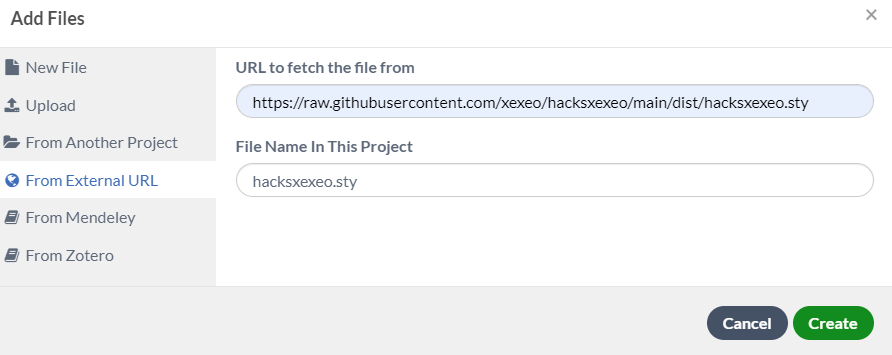
\includegraphics[width=0.9\linewidth]{images/overleaffileurl}
%    \caption{How to link a coop-writing.sty file in your project folder in Overleaf to the official distribution.}
%    \label{fig:overleaffileurl}
%\end{figure}
%
%
% \section{Package Options}
%
%
% Using the package allows the use of all macros and environments described in this manual, however, \textbf{if the options are not turned on, there will be no effect on the generated |pdf|}, since, by default, all options are false. 
%
% There are three types of options. The first type enables the visualization of the result of specific macros or environmnets, such as 
% the |cwdraft| environment. They are named \textit{command oriented options}. You can use many of them in the same time.
%
% The second type  represent a state
% of the text, which can be editing, submit, or publish, and some minor variations. They are named \textit{state oriented options}.
%
% The third type control other behaviors. They are named 
% \textit{behavior oriented options}
%
%
% If they appear together, state oriented commands have precedence over the others. However, the user should avoid mixing command and state oriented options. Also, most of the time, you should \textbf{use only one of the state oriented options.}
%
% It should be clear that the options have no impact on the availability of the macros and enviroments, they will be there for you to use, but the deeply affect their behavior. A macro that is very complex, such as |\cwauthor|, if one of options |comments| or |editing| is selected, is replaced by a simple version that do almost nothing.
%
% \subsection{Command oriented options}
% \begin{itemize}
%    \item |subjects|, \DescribeMacro{subjects}  enables the use of |\subject|, which is proposed as a paragraph heading describing its subject;
%    \item |comments|, \DescribeMacro{comments}  enables all editorial comments and the command |\pleasecite|;
%    \item |drafts|, \DescribeMacro{drafts}  enables the |\cwdraft| command;
%    \item |suggestions|, \DescribeMacro{suggestions}  enables the comments definided in the suggestion section of this text.
%    \item |anonymize|, \DescribeMacro{anonymize}   enables anonymization commands, and
%    \item |todos|, \DescribeMacro{todos}  enables the to do family of  commands.
%\end{itemize}
%
%\subsection{State oriented options}
% \begin{itemize}
% \item |submit|, \DescribeMacro{submit} enables the submit state. anonymization is on, subjects, comments, drafts and suggestions are off
% \item |noanonymize|, \DescribeMacro{noanonymize} disables anonymizations even in |submit| and |editing| options
% \item |publish|, \DescribeMacro{publish} disables all command oriented options, ignore suggestions.
% \item |acceptingpublish|, \DescribeMacro{acceptingpublish}  disables all command oriented options, accept suggestions
% \item |editing|, \DescribeMacro{editing}  enables |subjects|, |comments|, |drafts|, |anonymize|, and |suggestions|.
% \end{itemize}
%
%\subsection{Behavior oriented options}
%
% Some of this option are inherited from |ed|.
%
%
% \begin{itemize}
%    \item |nopdfbookmarks| will avoid adding bookmarks in the |pdf| file for all comments. The default behavior of |coop-writing| is adding them.
%    them.
%\end{itemize}
%
% \subsection{General behavior}
%
% The general behavior of this package is to provide different 
% ways of marking your text, for example with comments or to do notes, that can be totally supressed when desired. Mostly, this can be easilly done using one the the 3 main option states: |editing|, |submit|, and |publish|. 
%
% 
% Users should use the |editing| state most of the time. In this state, all
% markings will appear and the anonymization will be off.
%
% When submitting, the |submit| state will provide 
% a clean article, without any markings. Most of the times the article should be anonymized,
% but if this is not enforced, it is possible to use the options |submit| and |noanonymize| together. |publish| will never anonymize.
%
% The goal is to make the |submit| and |publish| documents states minimally
% invasive, to avoid any clash with publishers' styles. A clash will be considered a bug, and should be reported to the authors.
%
% If you use comments, there will be a lot of ``Marginpar moved'' warnings. 
% This is normal behavior, caused by the margin notes.
%
%
%\section{Version}
%
% It is possible that the user wants to know the version
% being used. We provide two commands for it.
%
% \DescribeMacro{\coopwritingversion}
% Provides the current version
%
% \DescribeMacro{\printcoopwritingversion}
% Provides name and version
%
%
% |\coopwritingversion| was used in the title of this article. The current version is \coopwritingversion. 
%
% If needed, the second macro prints also the name of the 
% package:
%
%|\printcoopwritingversion|
%
% will result in:
%
%\printcoopwritingversion
%
% Please state the version when reporting bugs.
%
%\section{Editorial comments}
%\label{sec:edcom}
%
% This is the main reason of this package.
%
% The idea is that not only users can make editorial comments on the 
% text they are writing, but they can also establish a dialog through those comments.
% I this package an editorial comment has 3 visual parts: an intervention in the 
% text, a margin note indicating this intervention, and a footnote explaining it\xexeo{This is the simplest form of an editorial note.}. Figure \ref{fig:editorialnotes} illustrate this behavior.
%
%
%\begin{figure}[tbh]
%    \centering
%    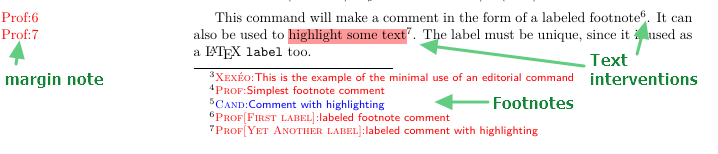
\includegraphics[width=0.8\linewidth]{images/editorialnotes}
%    \caption{How comments appear in the document when \texttt{editing} option is on.}
%    \label{fig:editorialnotes}
%\end{figure}
%
%
%
% \subsection{Creating authors}
%\label{sec:create} 
% \DescribeMacro{\cwnamedef}
% This macro creates a series of commands based on a desired base command name. The command name is, usually, the name of the author, of the editor, or a function in the work being done.
%
%  It must be given in the preamble of the \LaTeX document, i.e., before the |\begin{document}| declaration. It is usually done just after the |\usepackage{coop-writing}| line. 
% Its syntax is:
%
%|\cwnamedef| \marg{name}\marg{color}\marg{author-name}
%
%
% Where \meta{name} will be the base command name, which generates different commands by receiving sufixes, \meta{color} is the color to be used by all 
% comments and suggestions made by this author, and \meta{author-name} is the string to be used to represent the author.
%
% As an example, I usually declare myself as:
%
% |\cwnamedef{xexeo}{red}{Xexéo}|
%
% And, among other commands, |\xexeo| will be defined in such a way that it generates
% a footnote written in red, with a indicative margin note in the same color. Both will
% be identified with ``Xexéo''\xexeo{This is the example of the minimal use of an editorial command}.
%
%
% The \meta{name} and \meta{author-name} are different to support short command names and characters not supported in \LaTeX\  macros. Therefore, if you name is \textit{Gutemberg} you can create a family of commenting macros based on |\gut|, but use ``Gutemberg'' as your identifier.
%
%
% \DescribeMacro{\cwauthor}\DescribeMacro{\cweditor} 
% Two authors are pre-defined in the style, |cwauthor| and |cweditor|, to represent an author and an editor. 
%
% \subsection{Available commands}
%
% For each user created with command name \meta{name}, such as |cwauthor| and |cweditor|, used as example, the following commands are available.
%
% \subsubsection{Comments}
%
% \DescribeMacro{\<name>}
% \DescribeMacro{\cwauthor}
% \DescribeMacro{\cweditor}
% |\<name>| \oarg{selection}\marg{footnote comment} 
%
% |\cwauthor| \oarg{selection}\marg{footnote comment}
%
% |\cweditor| \oarg{selection}\marg{footnote comment}  
%
% These are the simplest commands, and will make a comment in the form of a identified footnote\cwauthor{Simplest footnote comment}. They can also be used to \cweditor[highlight some text]{Comment with highlighting}.
%
% \subsubsection{Labeled Comments}
%
% \DescribeMacro{\<name>r}
% \DescribeMacro{\cwauthorr}
% \DescribeMacro{\cweditorr}
% |\<name>r| \oarg{selection}\marg{footnote comment}\marg{label}
%
% |\cwauthorr| \oarg{selection}\marg{footnote comment}\marg{label}
%
% |\cweditorr| \oarg{selection}\marg{footnote comment}\marg{label}
%
% This command will make a comment in the form of a labeled footnote\cwauthorr{labeled footnote comment}{FirstLabel}. It can also be used to \cwauthorr[highlight some text]{labeled 
% comment with highlighting}{OtherLabel}. The label must be unique, and usually a single word, since it is used as a \LaTeX\  |\label| too. You can refer to this command using |\ref{cw:\meta{label}}|. For example, the comment \ref{cw:FirstLabel} would 
% be referenced as |\ref{FirstLabel}|.
%
%
% \subsection{Striked-throught comments}
%
% After using the editorial comments for a time we started to delete the old ones that
% represented fixed problems. However, we notice that some comments should be kept,
% even if solved.
% The solution was to create the striked-trought comments. They are easy to 
% use, just put an |x| after the command name.
% 
%
% \DescribeMacro{\<name>x}
% \DescribeMacro{\cwauthorx}
% \DescribeMacro{\cweditorx}
% |\<name>x| \oarg{selection}\marg{footnote comment} 
%
% |\cwauthorx| \oarg{selection}\marg{footnote comment} 
%
% |\cweditorx| \oarg{selection}\marg{footnote comment} 
%
% This command will make a comment in the form of a footnote\cweditorx{Simplest footnote 
% comment}, however the comment is striked through. It can also be used to \cwauthorx[highlight some text]{Comment with highlighting}.
%
% \DescribeMacro{\<name>rx}
% \DescribeMacro{\cwauthorrx}
% \DescribeMacro{\cweditorrx}
% |\<name>rx| \oarg{selection}\marg{footnote comment}\marg{label}
%
% |\cwauthorrx| \oarg{selection}\marg{footnote comment}\marg{label}
%
% |\cweditorrx| \oarg{selection}\marg{footnote comment}\marg{label}
%
%
% This command will make a comment in the form of a labeled footnote\cwauthorrx{labeled footnote comment}{Second label}, however the comment is striked through. It can also be used to \cwauthorrx[highlight some text]{labeled comment with highlighting}{New label}. The label must be unique, since it is used as a \LaTeX\  |label| too.
%
% \subsection{Text Modification - Suggestions}
% Sometimes one of the authors wants to insert, remove or edit some
% text, but he or she is not sure that every one will agree, therefore
% he or she can make a suggestion, that will appear with his or her color.
%
% \DescribeMacro{\<name>sug}
% \DescribeMacro{\cwauthorsug}
% \DescribeMacro{\cweditorsug}
% |\<name>sug|\oarg{comment}\marg{suggested text}
%
% |\cwauthorsug|\oarg{comment}\marg{suggested text}
%
% |\cweditorsug|\oarg{comment}\marg{suggested text}
%
%  This macro supports making a suggestion. It inserts text, using the color chosen 
% by the author. It is also possible to make a comment, but in this command the command 
% is the optional argument.
% 
% As example, in this paragraph the following text:
%
% \begin{verbatim}
%  \cwauthorsug{inserted text} will appears in the red, and it is 
% possible to \cweditorsug[I want to insert this]{use a comment}.
% \end{verbatim}
%
% generates:
%
%  \cwauthorsug{inserted text} will appears in the red, and it is 
% possible to \cweditorsug[I want to insert this]{use a comment}.
%
% \DescribeMacro{\<name>rem}
% \DescribeMacro{\cwauthorrem}
% \DescribeMacro{\cweditorrem}
% |\<name>rem|\oarg{comment}\marg{suggested removal}
%
% |\cwauthorrem|\oarg{comment}\marg{suggested removal}
%
% |\cweditorrem|\oarg{comment}\marg{suggested removal}
%
% This macro is used to suggest removals. 
%
% For example:
%
% \begin{verbatim}
% This is an example \cwauthorrem{that is quite good}. 
% Again, it is also possible to comment
% the \cwauthorrem[Repeated words]{the removal} removal.
%\end{verbatim}
%
% generates:
%
% This is an example \cwauthorrem{that is quite good}. 
% Again, it is also possible to comment
% the \cwauthorrem[Repeated words]{the removal} removal.
%
%
% \DescribeMacro{\<name>swap}
% \DescribeMacro{\cwauthorswap}
% \DescribeMacro{\cweditorswap}
% |\<name>swap|\oarg{comment}\marg{suggested removal}\marg{suggested insertion}
%
% |\cwauthorswap|\oarg{comment}\marg{suggested removal}\marg{suggested insertion}
%
% |\cweditorwap|\oarg{comment}\marg{suggested removal}\marg{suggested insertion}
%
% 
% This will work as the union of a removal and a suggestion. Actually, both are simplified forms of this command.
%
% For example:
%
% \begin{verbatim}
% \cwauthorswap{This should work like this.}%
% {This is an example of how the command should work.}%
% The following text is not a suggestion.
%\end{verbatim}
%
%
% generates:
%
% \cwauthorswap{This should work like this.}%
% {This is an example of how the command should work.}%
% The following text is not a suggestion.%
%
%
% \subsection{Putting more warning in text}
%
% It is possible to define a symbol, or any other thing, to appear
% before the superscript number that indicates the comment.
%
% This is done using \DescribeMacro{\cwsetcommwarn} the following command
% and syntax:
%
% |\cwsetcommwarn|\marg{symbol}
%
% Using package |marvosym|, the example:
%
% |\cwsetcommwarn{\Lightning}|
% \cwsetcommwarn{\Lightning}
%
% will change the behavior of editorial\xexeo{This comment superscript number should be preceeded by a \Lightning} comments to include the \Lightning\  symbol.
%
% You can remove the symbol by simply using |\cwsetcommwarn{}|
%
% \cwsetcommwarn{}
%
% It should be clear that |coop-writing| does not provide any font. If
% the user wants to use one font, like |marvosym|, he or she must import it with |\usepackage|.
%
% \subsection{A tip for using comments}
% 
% A student asked me to give a priority to my demands. This would
% make me add yet another set of commands, with more arguments.
% labels don't work because they must be unique to allow for being used as
% references. 
%
% The solution, however, is simple, special characters, such as $\star$, |$\star$|
% can be used and are highly efficient to communicate priority\xexeo{$\star$$\star$ Two stars are still low priority}.
%
% Using other fonts, more can be acomplished. For example, package 
%|marvosym| offers |\HollowBox|, \HollowBox, 
%|\Checkedbox|, \Checkedbox, 
%|\CrossedBox|, \CrossedBox, which can be 
% used to indicate that something should be done, is done or will not be 
% done.
%
% \section{Anonymization}
%
% Anonymization will provide commands to replace
% names and references by anonymous names and references.
% It will, by default, be enable only in the |submit| option
%
% There are 4 anonymization commands:
%
% \begin{itemize}
%   \item |\cwanon|\marg{text} \DescribeMacro{\cwanon}
%   \item |\cwanoncite|\oarg{cite-compatible-oarg}\marg{cite-compatible-arg} \DescribeMacro{\cwanoncite}
%   \item |\cwanoncitet|\oarg{citet-compatible-oarg}\marg{citet-compatible-arg} \DescribeMacro{\cwanoncitet}
%   \item |\cwanoncitep|\oarg{citep-compatible-oarg}\marg{citep-compatible-arg} \DescribeMacro{\cwanoncitep}
%\end{itemize}
%
% The alternative text used by anonymization commands can be configured with other commands:
%\begin{itemize}
%    \item |\cwdefanontext|\marg{replacement-text} \DescribeMacro{\cwdefanontext}
%    \item |\cwdefanoncitetext|\marg{replacement-text} \DescribeMacro{\cwdefanoncitetext}%    
%    \item |\cwdefanoncitettext|\marg{replacement-text} \DescribeMacro{\cwdefanoncitettext}
%\item|\cwdefanonciteptext|\marg{replacement-text} \DescribeMacro{\cwdefanonciteptext}
%\end{itemize}
%
% The example:
%
% \begin{verbatim}
% My name is \cwanon{Geraldo Xexéo}, and I read \cwanoncite{ed},
% \cwanoncitep[pags 1]{todonotes}, % \cwanoncitet{xcolor}.
% \end{verbatim}
%
% generates:
%
% My name is \cwanon{Geraldo Xexéo}, and I read \cwanoncite{ed},
% \cwanoncitep[pags 1]{todonotes}, % \cwanoncitet{xcolor}.
%
% Changing values, as in:
%
% \begin{verbatim}
% \cwdefanontext{Can't say}
% \cwdefanoncitetext{[0]}
% \cwdefanonciteptext{[X]}
% \cwdefanoncitettext{[Anon]}
% My name is \cwanon{Geraldo Xexéo}, and I read \cwanoncite{ed},
% \cwanoncitep[pags 1]{todonotes}, % \cwanoncitet{xcolor}.
% \end{verbatim}
% generates:
%
% \cwdefanontext{Can't say}
% \cwdefanoncitetext{[0]}
% \cwdefanonciteptext{[X]}
% \cwdefanoncitettext{[Anon]}
% My name is \cwanon{Geraldo Xexéo}, and I read \cwanoncite{ed},
% \cwanoncitep[pags 1]{todonotes}, % \cwanoncitet{xcolor}.
%
%
% \section{Draft environment}
% 
% \DescribeEnv{cwdraft}
% The |cwdraft| environment aims to allow writers to include text that is marked somehow as a draft\footnote{This was motivated because my students liked to hide text from me because ``it was only a draft'', but I need to have some way to measure if they were advancing. Marking text as a draft allowed them to be free of the fear of showing errors to me. I see it most as a psychological support to writing without fear of making mistakes. And, yes, you can still use footnotes and they will be correcly numbered}
%
% This environment is evolving, looking for a good way to signal the draft status, due to the different interactions with the packages it uses and user's packages.
% It has one optional parameter that names the draft. Its default value is ``Draft''
% If the |draft| option is not enabled, the text inside the title and the text inside the environment will not appear. The user should remember that some options will automatically turn on the |draft| option, such as the option |edicao|.
%
% The color of the title highlight can be changed with
%% \DescribeMacro{\cssetdraftcolor}
%
% |\cssetdraftcolor|\marg{color}
%
% The example:
%
%\begin{verbatim}
%\begin{cwdraft}[A draft title]
%This is the example of a draft.
%The title must be highlighted
%There must be a box around it.
%\end{cwdraft}
%
%\cwsetdraftcolor{blue}
%\begin{cwdraft}
%This draft has the default title.
%\end{cwdraft}
%\end{verbatim}
%
% generates:
%
%\begin{cwdraft}[A draft title]
% This is the example of a draft.
%
% The title must be highlighted
%
% There must be a box around it.
%\end{cwdraft}
%
%\cwsetdraftcolor{blue}
%\begin{cwdraft}
% This draft has the default title.
%\end{cwdraft}% 
%
%
% \section{Subjects}
%
% \DescribeMacro{\cwsubject}
% |\cwsubject|\oarg{color}\marg{text}
%
% These are supposed to help organizing a text by giving a ``title'' for each
% paragraph. 
%
% The idea here is that each paragraph should be about one and only one subject,
% and that reading these paragraph title will allow the authors to better understand
% what is being written and in which sequence.
%
% This feature was inspired by \citet{minto2009pyramid}.
%
% The example:
%
%\begin{verbatim}
% \cwsubject{Example of a subject}
% A subject is the main subject of a paragraph
%
% \cwsubject[pink]{A pink colored subject}
% You can use other colors, such as pink.%
%\end{verbatim}
%
%
% generates:
%
% \cwsubject{Example of a subject}
% A subject is the main subject of a paragraph
%
% \cwsubject[pink]{A pink colored subject}
% You can use other colors, such as pink.
%
% \section{Lists}
%
% \DescribeMacro{\listofcomment}\DescribeMacro{\listofcomment}\DescribeMacro{\listofsubject}Comments, citation demands and subjects can be list with these commands.
%
% The lists will only appear if their commands are enable (or in the all-enabling editing option).
% 
% They are usually put in the end of the file.
%
% \section{To dos}
%
% The |todo| command \DescribeMacro{\todo} is a much simpler version than 
% the one available in |todonotes|\xexeo{But it will grow in power with time}. It´s syntax is:
%
% |\todo|[inline]\marg{text}
%
% A todo without a inline option is equivent to a comment of
% author ``To do''\todo{This is how it works without the inline option}. With the option, the text will appear inside an orange box, as in the example below.
%
%
% The example:
%
%\begin{verbatim}
% \todo[inline]{This command can have other options, 
%based on other implementations of to do in different packages.}
%\end{verbatim}
%
% generates:
%
% \todo[inline]{This command can have other options, based on other implementations of to do in different packages}.
%
% It is possible to change the background color of the box using \DescribeMacro{\cwdefinetodocolor}. The idea, however, is that all to-dos should have the same color.
%
%  |\cwdefinetodocolor|\marg{color}. 
%
%
%
% The example:
%
%\begin{verbatim}
% \cwdefinetodocolor{yellow}
% \todo[inline]{This command can have other options, 
%based on other implementations of to do in different packages.}
%\end{verbatim}
%
% generates:
%
% \cwdefinetodocolor{yellow}
% \todo[inline]{This command can have other options, 
    %based on other implementations of to do in different packages.}
%
%
%\section{Warnings}
% This package uses another package that changes \LaTeX's standard behavior for summary and lists. When you use it, you must explicitly change pages with |\newpage| 
% before |\tableofcontents| or similar commands.
%
%
% \section{The commands in Portuguese}
% This section is in Brazilian Portuguese.
%
%\selectlanguage{brazilian}
% A Tabela \ref{tab:e2p} Mostra o mapeamento em inglês e português.  
% 
% \begin{table}[htb]
% \caption{Tradução dos comandos para português.}     
%\begin{tabular}{ccc}
%    \hline
%    Tipo & Inglês & Português \\
%    \hline
%    environment & |cwdraft| &|rascunho|\\
%    macro & |\cwnamedef| &|\cwautor|  \\
%    macro & |\cwsubject| & |\cwassunto|\\
%    macro & |\listofcomment| & |\listofcomentario|\\
%    macro & |\listofsubject| & |\listofassunto|\\
%    macro & |\listofcitationneeds| & |\listofcomentarioref|\\
%    macro & |\todo| & |\todo| \\
%    \hline
%\end{tabular}
% \label{tab:e2p}
% \end{table}
%
% \subsection{Opções em Português}
%
% As seguintes opções são aceitas em português, todas sem acentos ou cedilha: anonimizar, naoanonimizar, rascunhos, assuntos, comentarios, edicao, submeter, publicar, sugestoes, publicaraceitando. 
%\selectlanguage{english}
%\section{Comparision with other packages}
%
% It is interesting to compare this package with other 3:
% \begin{itemize}
%    \item |ed| has more features for commenting, and is more configurable, however it does not have colors.
% \item |todonotes| it does not have the identification of the commentator, which must be put by hand. It has more options too.
% \item |color-edits| does not support to do notes and drafts. 
% \end{itemize}
% 
% 
%
% \StopEventually{End of Code}
%
% \section{Implementation}
% This package was initially written in Portuguese. As it become more
% useful, it was translated to English. There are still some signs 
% of this in the code.
%
% \subsection{Access to the current version}
% We provide some macros for the user to know the version being used.
% \begin{macro}{\coopwritingversion}
% Provides current version of coop-writing
%    \begin{macrocode}
\newcommand{\coopwritingversion}{\cw@version}%
%    \end{macrocode}
% \end{macro}
% 
% \begin{macro}{\printcoopwritingversion}
% Provides package name and version
%    \begin{macrocode}
\newcommand{\printcoopwritingversion}{coop-writing v. \coopwritingversion}%
%    \end{macrocode}
% \end{macro}
%% 
%%
% \subsection{Option Processing}
% \subsubsection{Creating Options Variables used in ed}
% Some come from ed code and are being cleaned
%
%    \begin{macrocode}
\newif\ifshowednotes\showednotestrue% 
\newif\ifmargins\marginstrue%
\newif\ifednotebookmarks\ednotebookmarkstrue%
% \subsubsection{Creating Original Options Variables}
\newif\if@showcomentario\@showcomentariofalse%
\newif\if@naoanonimizar\@naoanonimizarfalse%
\newif\if@showdraft\@showdraftfalse%
\newif\if@showsubjects\@showsubjectsfalse%
\newif\if@showsugestao\@showsugestaofalse%
\newif\if@beanonymous\@beanonymousfalse%
\newif\if@showtodo\@showtodofalse%
\newif\if@modoedicao\@modoedicaofalse%
\newif\if@modosubmeter\@modosubmeterfalse%
\newif\if@modopublicar\@modopublicarfalse%
\newif\if@modopublicaraceitando\@modopublicaraceitandofalse%
%    \end{macrocode}
% \subsubsection{Portuguese Options}
%    \begin{macrocode}
\DeclareOption{rascunhos}{\@showdrafttrue}
\DeclareOption{comentarios}{\@showcomentariotrue}
\DeclareOption{anonimizar}{\@beanonymoustrue}
\DeclareOption{naoanonimizar}{\@naoanonimizartrue}
\DeclareOption{sugestoes}{\@showsugestaotrue}
\DeclareOption{assuntos}{\@showsubjectstrue}
\DeclareOption{edicao}{\@modoedicaotrue}
\DeclareOption{submeter}{\@modosubmetertrue}
\DeclareOption{publicar}{\@modopublicartrue}
\DeclareOption{publicaraceitando}{
    \@modopublicartrue 
    \@modopublicaraceitandotrue 
}
%    \end{macrocode}
% \subsubsection{English Options, inspired on ed package}
%    \begin{macrocode}
\DeclareOption{nopdfbookmarks}{\ednotebookmarksfalse}
%    \end{macrocode}
%
% \subsubsection{Original English Options}
%
%    \begin{macrocode}
\DeclareOption{comments}{\@showcomentariotrue}
\DeclareOption{anonymize}{\@beanonymoustrue}
\DeclareOption{noanonymize}{\@naoanonimizartrue}
\DeclareOption{suggestions}{\@showsugestaotrue}
\DeclareOption{subjects}{\@showsubjectstrue}
\DeclareOption{drafts}{\@showdrafttrue}
\DeclareOption{todos}{\@showtodotrue}
\DeclareOption{editing}{\@modoedicaotrue}
\DeclareOption{submit}{\@modosubmetertrue}
\DeclareOption{publish}{\@modopublicartrue}
\DeclareOption{acceptingpublish}{
    \@modopublicartrue 
    \@modopublicaraceitandotrue 
}
\ProcessOptions\relax
%    \end{macrocode}
% \subsubsection{Fixing the Super Options}
%    \begin{macrocode}
\if@modoedicao
\@showsubjectstrue
\@showdrafttrue
\@showcomentariotrue
\@showsugestaotrue
\@beanonymoustrue
\@showtodotrue
\fi
\if@modosubmeter
\@showsubjectsfalse
\@showdraftfalse
\@showcomentariofalse
\@showsugestaofalse
\@beanonymoustrue
\@showtodofalse
\fi
\if@naoanonimizar
\@beanonymousfalse
\fi
\if@modopublicar
\@showsubjectsfalse
\@showsugestaofalse
\@showdraftfalse
\@showcomentariofalse
\@beanonymousfalse
\@showtodofalse
\fi%
\if@showtodo
\@showcomentariotrue
\fi
%    \end{macrocode}
% \subsection{Required Packages}
% Packages that are always required
%\begin{itemize}
%    \item xcolor - used to support colors 
%    \item soulutf8 - this is a variation of soul, used for highlighting
% \item ulem - used to support strikethrought\todo{I must complete this explanation list}
% \item tocloft - used to support modifications in lists and tocs
% \item mdframed - used to support boxes for todos and drafts
% \item iflang - used to check if language is loaded and define new words not in Babel
%\end{itemize}
%    \begin{macrocode}
\RequirePackage{xcolor}
\RequirePackage{soulutf8}
\RequirePackage[normalem]{ulem}
\RequirePackage{tocloft}
\RequirePackage{etoolbox}
\RequirePackage{environ}
\RequirePackage{xstring}
\RequirePackage{csquotes}
\RequirePackage{mdframed}
%    \end{macrocode}
% \subsection{Optional Packages}
% Package that are required only sometimes
%    \begin{macrocode}
\ifshowednotes%
\else%
\RequirePackage{verbatim}%
\fi%
%    \end{macrocode}
% Checking if babel is loaded, use iflang
%    \begin{macrocode}
\@ifpackageloaded{babel}%
{%  \message{Babel Loaded!}%
    \RequirePackage{iflang}%
}{%
    \message{Babel not detected!}%
}%
%    \end{macrocode}
%    \begin{macrocode}
% |hyperref| must always be the last
\ifednotebookmarks\RequirePackage{hyperref}\fi
%    \end{macrocode}
% \subsection{Color related variables}
%    \begin{macrocode}
\newcommand{\cor@prof}{red}%
\newcommand{\cor@cand}{blue}%
\newcommand{\cor@subject}{green}%
\newcommand{\cor@citar}{purple}%
\newcommand{\cor@hldraft}{yellow}%
%    \end{macrocode}
%
% \subsection{I18N Almost Using Babel}
% We can detect if babel is enable and allow for some languages.
% If you want to use another language, you must set new values
% for the command |\cwdrafttitle|.
% I really thought that it was possible to do something smarter with babel, for example using |\setlocalecaption|, but no attempt worked out was I wanted.
%
% There are some packages, as |translator| that can be useful
% but up to now this seems to be the easiest way of doing it.
%
% The advantage of this way is that any user can |\renewcommand{\cwdrafttitle}{some text}|.
%    \begin{macrocode}
\def\cwdrafttitle{Standard Draft}%
\def\cwcommentstitle{Standard List of Comments}%
\def\cwsubjtitle{Standard List of Subjects}%
\def\cwcitationstitle{Standard List of Citation Needs}%
\def\cwpleasecitetext{Plese cite}%
\def\cwpleasecitemessage{something to support this information}%
\def\cwpleasecitemarginnote{Cite}%
%
\@ifpackageloaded{babel}%
{%
    \IfLanguageName{brazilian}%
    {%
        \def\cwdrafttitle{draft}%
        \def\cwcommentstitle{Lista de Comentários}%
        \def\cwsubjtitle{Lista de Assuntos}%
        \def\cwcitationstitle{Necessidades de Citação}%        
        \def\cwpleasecitetext{Favor citar}%
        \def\cwpleasecitemessage{alguma coisa que suporte este texto}%
        \def\cwpleasecitemarginnote{Citar}%
    }{}%
%    
    \IfLanguageName{portuguese}%
    {%
        \def\cwdrafttitle{draft}%
        \def\cwcommentstitle{Lista de Comentários}%
        \def\cwsubjtitle{Lista de Assuntos}%
        \def\cwcitationstitle{Necessidades de Citação}%        
        \def\cwpleasecitetext{Favor citar}%
        \def\cwpleasecitemessage{alguma coisa que suporte este texto}%
        \def\cwpleasecitemarginnote{Citar}%
    }{}%
%    
    \IfLanguageName{english}%
    {%
        \def\cwdrafttitle{Draft}%
        \def\cwcommentstitle{List of Comments}%
        \def\cwsubjtitle{List of Subjects}%
        \def\cwcitationstitle{List of Citation Needs}%
        \def\cwpleasecitetext{Plese cite}%
        \def\cwpleasecitemessage{something to support this information}%
        \def\cwpleasecitemarginnote{Cite}%
    }{}%
}%
{}%
%    \end{macrocode}
% \subsection{ed inspired code}
% This code, inspired in the |ed| package, makes the basic mechanism for 
% inserting comments as footnotes with an observation in the margin.
% As an adition to |ed|, it support colors and some text
% before the superscript number in the text
% \begin{macro}{cwnotecounter}
% Setting up the counter that gives the number of the footnote
%    \begin{macrocode}
\newcounter{cwnotecounter}%
%    \end{macrocode}
% \end{macro}
% \subsubsection{The footnote}
% Format for the text 
%    \begin{macrocode}
\newcommand\cw@noteshape{\sffamily}%
%    \end{macrocode}
% Defining the variable that holds the color to be printed.
% |soul| made it quite complex, global variable is not the best programming technique, but it works.
%    \begin{macrocode}
\def\cw@currentcolor{black}%
%    \end{macrocode}
%% footnote indicador e rótulo
% \begin{macro}{\cw@foot}
%
% This macro write the text in the footnote using with standard \LaTeX\ |\footnotetext|
%
% It uses counter |cwnotecounter| in arabic. 
% It prints the footnote using the currently defined color (That is a global variable, setted up elsewehre. This is not good programming practice,
% but it turned out to be the easiest way of doing it in \LaTeX without more and more arguments.)
%
% Syntax: |\cw@foot|\marg{footnote-text}\marg{author-name}\marg{label}
%
%
% If this is a labeled note, it will create a \LaTeX label on the format
%
% |cw:|\meta{label}
%
% That can be used in a |\ref| command.
%
%    \begin{macrocode}
\newcommand\cw@foot[3]% 
{%
\def\@test{#3}% @test just checks if argument #3 exists
\footnotetext[\arabic{cwnotecounter}]% 
{%
{\scshape{\textcolor{\cw@currentcolor}{#2}}%
\if\@test%
\@empty%
\else%
\label{cw:#3}%
\textcolor{\cw@currentcolor}{[#3]}% if \meta{label} is not empty
\fi%
\textcolor{\cw@currentcolor}{:}}% 
\cw@noteshape\textcolor{\cw@currentcolor}{#1}}%
}%
%    \end{macrocode}
% \end{macro}
% \begin{macro}{\cw@mark}
% This macro generates the footnote mark with standard \LaTeX\ 
% |\footnotemark|
%    \begin{macrocode}
\def\cw@mark@style#1{#1}%
\newcommand\cw@mark[1]{\cw@mark@style{\footnotemark[#1]}}%
%    \end{macrocode}
% \end{macro}
% \begin{macro}{\cw@beforemarksymbol}
% \begin{macro}{\cwsetcommwarn}
%
%  These macros control the symbol (or any text) that can
%  appear before the footnotemark
%
%  |\cwsetcommwarn|\marg{symbol}
%
%  \meta{symbol} can be of any length, but we suggest only one
% character. It can be empty, what is the default option,
% and will print nothing at that point.
%
%    \begin{macrocode}
\newcommand{\cw@beforemarksymbol}{}%
\newcommand{\cwsetcommwarn}[1]{\def\cw@beforemarksymbol{#1}}%
%    \end{macrocode}
%
% \end{macro}
% \end{macro}
%
% \begin{macro}{\cw@footnote}
%
% This macro actually makes the footnote symbol, mark and text
%  
% Syntax is:
%
% |\cw@footnote|\marg{text}\marg{name}\marg{label}
%
% \meta{label} can be empty, but must be present
%
% It is in this macro that symbol, number and footnote mark
% end up in the document. 
%
% This command also changes the color of footnote mark
%
%    \begin{macrocode}
\newcommand\cw@footnote[3]{%
\renewcommand\@makefnmark{\hbox{\@textsuperscript{\normalfont\color{\cw@currentcolor}\@thefnmark}}}%
\textcolor{\cw@currentcolor}{\cw@beforemarksymbol\cw@mark{\arabic{cwnotecounter}}}%
\cw@foot{#1}{#2}{#3}%
}%
%    \end{macrocode}
% \end{macro}
% \subsubsection{The margin note}
%
% This macro builds the margin note.
%
%    \begin{macrocode}
\newcommand\cw@margin[1]{%
\ifmargins%
\marginpar{\textcolor{\cw@currentcolor}{#1}}%
\fi%
}%
%    \end{macrocode}
% \begin{macro}{\Cw@note}
% Basic function to build the comment
% 
% |\Cw@note|\marg{text}\marg{name}\marg{label}
%
% If not label, it must be empty
%
%
%    \begin{macrocode}
\newcommand\Cw@note[3]% text, name, label
{%
\addtocounter{cwnotecounter}{1}%
\ifshowednotes%
\cw@footnote{#1}{#2}{#3}%
\ifednotebookmarks%
\belowpdfbookmark{#2: #1}{cwnotepdfbm.\thecwnotecounter}%
\fi%
\fi}%
%    \end{macrocode}
% \end{macro}
% More functions for doing the editorial note
%    \begin{macrocode}
\newcommand\cw@note[4]% text, type, label, margin
{\Cw@note{#1}{#2}{#3}%
\ifshowednotes%
\cw@margin{#4:\arabic{cwnotecounter}}%
\fi}%
\newcommand\cwnote@label{Editor}%
\newcommand\cwnote@margin{Ed}%
\newcommand\cwnotelabel[1]{\def\cwnote@label{#1}}%
\newcommand\cwnotemargin[1]{\def\cwnote@margin{#1}}%
\newcommand{\Cwnote}[2][]{\Cw@note{#2}\cwnote@label{#1}}%
%
\newcommand{\cwnote}[3][]{%
\def\cw@currentcolor{#3}%
\cw@note{#2}%
\cwnote@label{#1}%
\cwnote@margin%
}%
%%%https://tex.stackexchange.com/questions/30483/how-can-i-check-in-latex-or-plain-tex-whether-a-command-exists-by-name
%% as opções comentario, assuntos e anonimizar
%% CORES
%    \end{macrocode}
% \begin{macro}{\corleve}
% Make a color lighter for later use in highlightings
% This code is more complex than it shuould be because o |soulutf8|'s package |\hl| behavior. Solution found in: 
% \url{https://tex.stackexchange.com/questions/410295/soul-color-transparency}
%    \begin{macrocode}
\newcommand{\cor@suavizacao}{40}%
\newcommand{\corleve}[1]{#1!\cor@suavizacao!white}
%    \end{macrocode}
% \end{macro}
% \begin{macro}{\cw@hll}
% Light highlight makes a |\hl| that is lighter
%    \begin{macrocode}
\newcommand{\cw@hll}[2]% % Depedendo do soulutf8
{\colorlet{x@coraqui}{\corleve{#1}}%
\sethlcolor{x@coraqui}%
\hl{#2}%
}%
%    \end{macrocode}
% \end{macro}
% Isolating cwnote
%    \begin{macrocode}
%% rótulo texto cor indicador
\newcommand{\cw@cwnote}[4][]{%
\cwnotelabel{#4}%
\cwnotemargin{#4}%
\cwnote[#1]{#2}{#3}%
}%
%    \end{macrocode}
% \subsection{Anonymization}
% Will write anonymous or cite anonymous. 
% The user has a way to configure the citation as he or she wants.
% \begin{macro}{\cw@anontext}
% \begin{macro}{\cw@anoncitetext}
% \begin{macro}{\cw@anonciteptext}
% \begin{macro}{\cw@anoncitettext}
%
% Default values for anonymous citation.
%
%    \begin{macrocode}
%
\newcommand{\cw@anontext}{Anonymous}
\newcommand{\cw@anoncitetext}{(Anonymous, Year)}%
\newcommand{\cw@anonciteptext}{(Anonymous, Year)}%
\newcommand{\cw@anoncitettext}{Anonymous (Year)}%
%    \end{macrocode}
% \end{macro}
% \end{macro}
% \end{macro}
% \end{macro}
% \begin{macro}{\cwdefanontext}
% \begin{macro}{\cwdefanoncitetext}
% \begin{macro}{\cwdefanonciteptext}
% \begin{macro}{\cwdefanoncitettext}
% These macros allow to define how anonymous citations will appear is
% anonymous mode is activated. For exemplo, one can change all the
% citation formats to |[0]|.
%    \begin{macrocode}
\newcommand{\cwdefanontext}[1]{\renewcommand{\cw@anontext}{#1}}%
\newcommand{\cwdefanoncitetext}[1]{\renewcommand{\cw@anoncitetext}{#1}}%
\newcommand{\cwdefanonciteptext}[1]{\renewcommand{\cw@anonciteptext}{#1}}
\newcommand{\cwdefanoncitettext}[1]{\renewcommand{\cw@anoncitettext}{#1}}%
%    \end{macrocode}
% \end{macro}
% \end{macro}
% \end{macro}
% \end{macro}
%    \begin{macrocode}
\if@beanonymous
\newcommand{\cwanon}[1]{\cw@anontext}%
\newcommand{\cwanoncite}[2][]{\cw@anoncitetext}%
\newcommand{\cwanoncitep}[2][]{\cw@anonciteptext}%
\newcommand{\cwanoncitet}[2][]{\cw@anoncitettext}%
\else
\newcommand{\cwanon}[1]{#1}%
\newcommand{\cwanoncite}[2][]{\cite[#1]{#2}}%
\ifdef{\citep}{\newcommand{\cwanoncitep}[2][]{\citep[#1]{#2}}}{\newcommand{\cwanoncitep}[2][]{\citep[#1]{#2}}}%
\ifdef{\citet}{\newcommand{\cwanoncitet}[2][]{\citet[#1]{#2}}}{\newcommand{\cwanoncitet}[2][]{\citet[#1]{#2}}}%
\fi%|
%    \end{macrocode}
% \subsection{Subjects}
% The idea of subjects is to have one subject for each paragraph
% Currently is just a list of subjects and and a highlight
%    \begin{macrocode}
\if@showsubjects
\newcommand{\listsubject}{\cwsubjtitle}%
%% cria a lista, depende do pacoto tcloft
\@ifundefined{chapter}
{\newlistof[section]{subject}{aaa}{\listsubject}}
{\newlistof[chapter]{subject}{aaa}{\listsubject}}%
%%
\newcommand{\cwsubject}[2][\cor@subject]{%
\refstepcounter{subject}%
\sethlcolor{#1}%
\hl{#2}%
\par%
\addcontentsline{aaa}{subject}{\protect\numberline{\thesubject}{#2}}%
}%
\setlength{\cftsubjectnumwidth}{2.5em}%
\else%
\newcommand{\listofsubject}{}%
\newcommand{\cwsubject}[2][]{}%
\fi%
%    \end{macrocode}
% \subsection{Editorial Comments}
% The main subject of this package
%    \begin{macrocode}
\if@showcomentario
%% Resolve a lista de comentários
\newcommand{\listcomentario}{\cwcommentstitle}%
%% cria a lista
\@ifundefined{chapter}
{\newlistof[section]{comentario}{ccc}{\listcomentario}}
{\newlistof[chapter]{comentario}{ccc}{\listcomentario}}%%
%%
%% Comentador genérico - parte I
%% faz o cwnote e soma na lista
%% []rótulo], texto , cor, indicador
\newcommand{\cw@comentar}[4][]{%
\ifstrempty{#4}{%
% rótulo texto cor indicador
\cw@cwnote[#1]{#2}{#3}{Comentário}% faz a nota de rodapé do ed
\addcontentsline{ccc}{comentario}{\protect\numberline{\thecomentario}{#2}}%
}%
{%
\cw@cwnote[#1]{#2}{#3}{#4}%
\addcontentsline{ccc}{comentario}{\protect\numberline{\thecomentario}{#4: #2}}%
}%
}%
%% comentador genérico, parte II
%% faz o highlight , soma o step e comenta
%% [texto hl] footnote cor indicator
\newcommand{\cw@comment}[4][]{%
\refstepcounter{comentario}% soma um ao contador
\cw@hll{#3}{#1}% ver subfunção de impressão com hl
\cw@comentar{#2}{#3}{#4}%
}%
%%
%%
\newcommand{\cw@xcomment}[4][]{%
\refstepcounter{comentario}% soma um ao contador
\cw@hll{#3}{#1}% ver subfunção de impressão com hl
\cw@comentar{\sout{#2}}{#3}{#4}%
}%
%%
%%
%% comentador genérico com rótulo
%% [texto hl] footnote cor  indicator rótulo
\newcommand{\cw@commentLabeled}[5][]{%
\refstepcounter{comentario}%
\cw@hll{#3}{#1}%
\cw@comentar[#5]{#2}{#3}{#4}%
}%
%%
%% [texto hl] footnote cor  indicator rótulo
\newcommand{\cw@xcommentLabeled}[5][]{%
\refstepcounter{comentario}%
\cw@hll{#3}{#1}%
\cw@comentar[#5]{\sout{#2}}{#3}{#4}%
}%
%%
\setlength{\cftcomentarionumwidth}{2.5em}
\else
\newcommand{\cw@comentar}[4][]{}%
\newcommand{\listofcomentario}{}%
%% não pode perder o texto comentado
\newcommand{\cw@comment}[4][]{#1}%
\newcommand{\cw@commentLabeled}[5][]{#1}%
\newcommand{\cw@xcomment}[4][]{#1}
\newcommand{\cw@xcommentLabeled}[5][]{#1}%
\fi%|
%    \end{macrocode}
% \subsection{Suggestions, Removes and Changes}
%    \begin{macrocode}
%% comentário, cor, indicador, textovelho, cor velho, textonovo, cor novo
%% Em modo publicar coloca o textovelho
\if@showsugestao
\newcommand{\cw@gensug}[7][Uma proposta]{%
\textcolor{#5}{\sout{#4}}% CORRIGINDO AQUI
\textcolor{#7}{#6}%
\if@showcomentario%
\ifstrempty{#1}{}%
{\refstepcounter{comentario}%
\cw@comentar{#1}{#2}{#3}%% [rótulo], cor , footnote , indicador
}%
\fi%
}%% [rótulo], cor , footnote , indicador
\else%
\if@modopublicaraceitando
\newcommand{\cw@gensug}[7][]{#6}%
\else%
\newcommand{\cw@gensug}[7][]{#4}%
\fi%
\fi%
%    \end{macrocode}
% \subsection{Citations Needed}
% One common error of students is not to cite correctly.
% Citation errors are so common that I decided to provide the option to have an optional list just for them.
% They are enable together with commentaries, users can use them or not.
%    \begin{macrocode}
\if@showcomentario%
\newcommand{\listcomentarioref}{\cwcitationstitle}%
\@ifundefined{chapter}{ \newlistof[section]{comentarioref}{ccr}{\listcomentarioref}}{\newlistof[chapter]{comentarioref}{ccr}{\listcomentarioref}}%
\else%
\newcommand{\listofcomentarioref}{}%
\fi%
\if@showcomentario%
\newcommand{\cw@commentref}[3][]{%
\refstepcounter{comentarioref}%
\cw@hll{#3}{#1}%
\cw@cwnote{#2}{#3}{\cwpleasecitemarginnote}%
\addcontentsline{ccr}{comentarioref}{\protect\numberline{\thecomentarioref}{#2}}%
}%
\setlength{\cftcomentariorefnumwidth}{2.5em}%
\else%
\newcommand{\cw@commentref}[3]{}%
\fi%
\if@showcomentario
\newcommand{\favorcitar}[1][\cwpleasecitemessage]{%
\cw@commentref{\cwpleasecitetext\  #1}{\cor@citar}}%
\else%
\newcommand{\favorcitar}[1][]{}%
\fi%
%    \end{macrocode}
% \subsection{Draft}
% \begin{environment}{cwdraft}
% This enviroment creates a boxed text, with title used as a first parameter
% It uses package |mdframed| to create the frame.
% If draft is turned off as an option, it supress everything inside the body.
% Due to problems with soul accepting |\cwdrafttitle| we use
% |\colorbox| to support multiple languages if default title is
% used
%    \begin{macrocode}
\if@showdraft%
\NewEnviron{cwdraft}[1][]{%
\ifstrempty{#1}%
{\colorbox{\corleve{\cor@hldraft}}{\textbf{\cwdrafttitle}}}%
{\cw@hll{\cor@hldraft}{\textbf{#1}}}%
\newline%
\BODY%
}%
{}%
\surroundwithmdframed{cwdraft}%
\else%
\NewEnviron{cwdraft}[1][]{}{}%
\fi%
%    \end{macrocode}
% \begin{macro}{\cwsetdraftcolor}
% Sets the color that highlights the draft title
% 
%    \begin{macrocode}
% 
\newcommand{\cwsetdraftcolor}[1]{\def\cor@hldraft{#1}}
%
%    \end{macrocode}
% \end{macro}
% \end{environment}
% \subsection{Powerful command to create editors and authors}
% This allows for many types of comments. This was the reason I started
% using a front-end to |ed|, and later decided to use colors, that |ed| dones not support.
% If I had known of |color-edits|, maybe this package was never done. I actually implemented the same functionalities without knowing about that package. One day, looking for other editorial packages that used editorial symbols, I found |color-edits|, but it was too late, I was already hooked on \LaTeX\  programming addiction.
%% nome do autor, cor, identificador
% \begin{macro}{\cwautor}
%    \begin{macrocode}
\newcommand{\cwautor}[3]{%
%% cwcomment - texto a hl, cor, comentário, indicador de pessoa
\expandafter\newcommand\csname#1\endcsname[2][]%
{%
\cw@comment[##1]{##2}{#2}{#3}}%
% [texto a marcar], cor , comentário, palavra, rótulo
\expandafter\newcommand\csname#1r\endcsname[3][]%
{\cw@commentLabeled[##1]{##2}{#2}{#3}{##3}}%
%% cortados
\expandafter\newcommand\csname#1x\endcsname[2][]%
{%
%% Comentários
\cw@xcomment[##1]{##2}{#2}{#3}}%
%% [texto a marcar], cor , comentário, palavra, rótulo
\expandafter\newcommand\csname#1rx\endcsname[3][]%
{\cw@xcommentLabeled[##1]{##2}{#2}{#3}{##3}}%
%% sugestões
\expandafter\newcommand\csname#1sug\endcsname[2][]%
{\cw@gensug[##1]{#2}{#3}{}{#2}{##2}{#2}}%
\expandafter\newcommand\csname#1rem\endcsname[2][]%
{\cw@gensug[##1]{#2}{#3}{##2}{#2}{}{#2}}
\expandafter\newcommand\csname#1troca\endcsname[3][]%
{\cw@gensug[##1]{#2}{#3}{##2}{#2}{##3}{#2}}%
\expandafter\newcommand\csname#1swap\endcsname[3][]%
{\cw@gensug[##1]{#2}{#3}{##2}{#2}{##3}{#2}}%
}%
%    \end{macrocode}
% \end{macro}
% \begin{macro}{\cwauthor}
% \begin{macro}{\cweditor}
% These are the two standard users. 
%    \begin{macrocode}
\cwautor{cwauthor}{red}{Author}
\cwautor{cweditor}{blue}{Editor}
%    \end{macrocode}
% \end{macro}
% \end{macro}
% \subsection{To do notes}
% This was developed because some of my students started a text using |todonotes|, before being aware of my package, therefore I need to have some compatibility to make de change. With time it became useful and I will try to make something better in the future.
% \begin{macro}{\todo}
% If option inline is not used, it is only a front-end to 
% an editorial comment for a user called ``To do''. If it is used, it tries to simulate
% the simplest behavior of |todonotes| package.
% In the future this can be enhanced, since package |mdframe| is very powerful.
% If the non-inline version is used, the to do note will not appear in the List of Commentaries.\xexeo{It would be nice to check if todonotes is load and just use it}
%    \begin{macrocode}
\newcommand{\cw@todobackgroundcolor}{orange}%
\cwautor{cw@todoauthor}{orange}{To do}%
\if@showtodo%
\newcommand{\todo}[2][comentar]{%
\IfEq{inline}{#1}%
{%
\begin{mdframed}[backgroundcolor=\cw@todobackgroundcolor]
#2%
\end{mdframed}%
}%
{%
\cw@todoauthor{#2}%
}%
}%
\else%
\newcommand{\todo}[2]{}%
\fi%
%    \end{macrocode}
% \end{macro}
% \begin{macro}{\cwdefinetodocolor}
% Allows the definition of a background color for todo notes.
%    \begin{macrocode}
\newcommand{\cwdefinetodocolor}[1]{\renewcommand{\cw@todobackgroundcolor}{#1}}%
%    \end{macrocode}
% \end{macro}
%  \subsection{Portuguese/English, or inverse translation table}
% These next lines of code made easy to convert this package to English, because it was written in Portuguese, for Brazilian researchers.
% Some commands were rewritten in English with time, such as |rascunho|, but the Portuguese version will always be maintained, while other were translated using only his mechanism.
%    \begin{macrocode}
\let\rascunho=\cwdraft%
\let\cwassunto=\cwsubject%
\let\pleasecite=\favorcitar%
\let\cwnamedef=\cwautor%
\let\listofcomments=\listofcomentario%
\let\listofcitationneeds=\listofcomentarioref%
\let\listofassunto=\listofsubject%
%    \end{macrocode}
% \Finale
%
% \endinput
% Local Variables:
% mode: doctex
% TeX-master: t
% End:
